% ビットレートの要件 ... double*3を入れるには200bpsは必須
Considering practical usage of annotations for content editing, we thought that in minimum 200 bps is required as the data rate of watermarking, because if an user wants to record a value of a sensor (e.g. GPS) consists of two or three double-precision floating-point number every second, 8 (bit/byte) * 8 (bytes) * 3 = 192 (bits) must be able to be embedded in one second.
% ヘッダや透かし間ギャップを考慮すると400bpsは欲しい
Taking an overhead from packet header/footer and required gap between watermarks for stability of decoding into account, at least 400 bps is desirable as the gross bit rate for our watermarking technique.

% 非可聴域を用いて変調を行うに当たって、我々は予備調査を行った
We conducted a preliminary study to choose appropriate method for modulating digital data in inaudible frequency range that satisfies this requirement.
In this study, we implemented watermark transmitters and demodulators for two modulation methods and roughly evaluated their performance by using them in real hardware setup.

% 一方はOFDM
The first method uses orthogonal frequency-division multiplexing (OFDM) to make full use of available bandwidth over 18 kHz, following the idea of Matsuoka's {\it Acoustic OFDM} \cite{matsuoka2008acoustic}.
% OFDMとは
OFDM is a specialized variety of frequency-division 
multiplexing (FDM) that uses multiple sub-carriers with different frequencies to transmit information in parallel.
A signal of OFDM is synthesized by composing signals of all sub-carrier waves.
% OFDMの特徴
In OFDM, carrier frequencies are selected in orthogonal, in other words, signals of sub-carriers are independent of and do not interfere each other.
This characteristic realize closer spaces between carrier frequencies and transmitting larger number of sub-carriers than ordinary FDM in certain bandwidth, therefore using OFDM increases bit rate of transmission.
% 用いた条件
In our preliminary study, eight sub-carriers with equally spaced frequencies between 17900 Hz and 20000 Hz were used to send octet bits in one signal, and each sub-carrier signal was modulated using differential binary phase shift keying (D-BPSK) in 100 bps (10 milliseconds per unit signal).
In total, gross bit rate was 800 bps in the condition, which satisfies the requirement mentioned above enough.

% 他方はDTMF
The other method also employs multiple sub-carriers with different frequencies to transmit information more than a bit in a unit signal, however it uses dual-tone multiple-frequency (DTMF) technique for multiplexing.
A unit signal of DTMF is a composition of just two sinusoidal waves of different frequencies, and combination of the two frequencies represents the value of the signal.
Since the number of possible signal varieties of $n$-frequency DTMF is $_n C _2$, at most $\log_2 {}_n C _2$ bits can be sent in a signal.
% DTMFの特徴
In DTMF, the amount of information can be sent in a signal is smaller than OFDM if the number of sub-carriers are same, however signal intensity of each frequency can be much stronger when that of composed signal is restricted by hardware constraints, because only two sub-carriers are composed simultaneously.
% 用いた条件
In this study, we used seven sub-carriers with equally spaced frequencies between 17600 Hz and 20000 Hz for DTMF. Since $_7 C _2$ is 21, 16 combinations among all pairs of seven frequencies were used to represent four bits per signal.
The length of a signal was set 10 ms, the same as that of first method.
In total, gross bit rate was 400 bps in the condition.

% 実験結果
As the result of the study, we found the first method with OFDM not suited for our purpose because of its worse embedding reliability besides its higher bit rate.
Extraction of watermarks is instable in the method due to the weaker intensity of each sub-carriers because of small output power of a speaker of a smartphone.
% 大きいスピーカーを使えば解決するが、今回の目的には適切ではない
However the embedding performance would be gained enough if a loud speaker with enough power could be available, using OFDM seemed not to be appropriate choice since small hardware constraint is required in our purpose.
% DTMFを使うことにした
In conclusion, we decided to use DTMF in our watermarking scheme appreciating its higher reliability.

% スペクトログラム
\begin{figure}[htbp]
 \begin{center}
  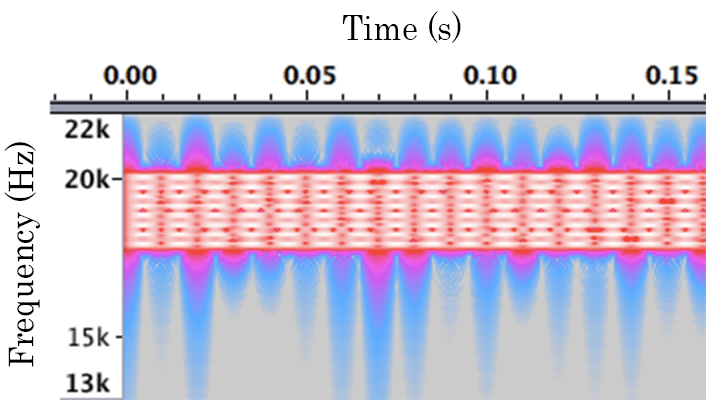
\includegraphics[height=35mm]{watermarking_ofdm.png}
  \hspace{5mm}
  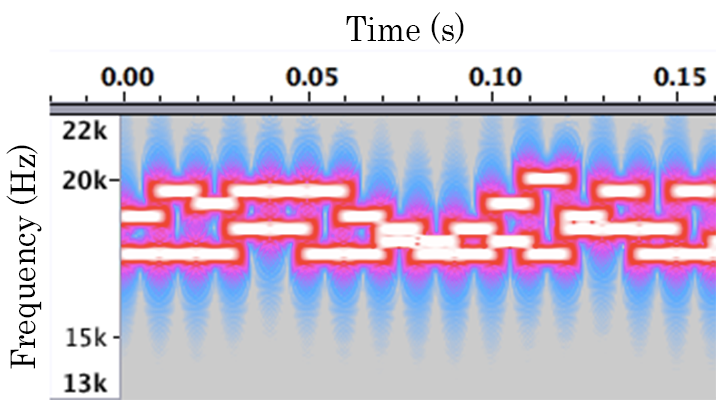
\includegraphics[height=35mm]{watermarking_dtmf.png}
 \end{center}
 \caption{Left: The spectrogram of a OFDM modulated watermark. Right: That of a DTMF modulated watermark.}
 \label{fig:watr_spec}
\end{figure}
